\section{Low-Compute Benchmark and Experiments}

\paragraph{Environments.}
The benchmark uses four deterministic CPU environments. The point mass is a positive control with $J=I$. The nonholonomic car exposes sideways visual futures that are locally impossible. The two-link arm uses an analytic end-effector Jacobian and action limits. The planar pusher has a contact-dependent Jacobian, so object motion before contact is non-actionable.

\begin{figure}[t]
\centering
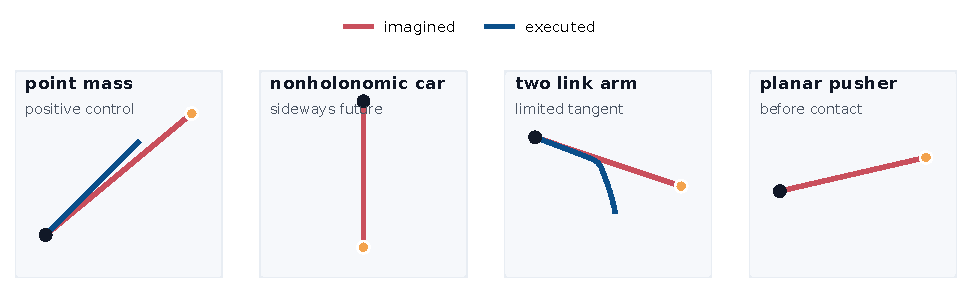
\includegraphics[width=0.95\linewidth]{figures/fig3_environment_grid.pdf}
\caption{Representative imagined trajectories and rollouts under recovered controls. The environments isolate different reasons a plausible representation future can fail under the executing body.}
\label{fig:envs}
\end{figure}

\paragraph{Generated futures.}
We use controlled future generators rather than large video models: straight-line interpolation, noisy splines, passive smoothness priors, scripted rollouts, and intentionally non-actionable futures. These generators are proxies for generated visual futures and are not claimed to match real video-model distributions.

\paragraph{Experiment 1: constructive counterexample.}
The car example in Proposition 1 is implemented directly. A sideways future has the same endpoint smoothness as a forward future under passive scoring, but the residual rejects it because the displacement lies outside the car's local tangent set.

\paragraph{Experiment 2: failure prediction.}
For each candidate, we compute residuals, recover controls, roll out the true environment, and mark failure when the executed path diverges from the imagined path. Table~\ref{tab:failure} reports the actionability score. In the saved CSVs, it is compared to smoothness, path length, action norm, passive negative log-likelihood proxy, and random score.

\begin{table}[t]
\centering
\caption{Failure prediction with the actionability residual. Higher scores predict execution failure.}
\label{tab:failure}
\begin{tabular}{lccc}\toprule
Environment & AUROC & AUPRC & Acc.\\\midrule
nonholonomic car & 1.000 & 1.000 & 0.900\\
planar pusher & 1.000 & 1.000 & 0.900\\
point mass & 1.000 & 1.000 & 0.900\\
two link arm & 0.990 & 0.966 & 0.811\\
all & 0.989 & 0.989 & 0.917\\
\bottomrule\end{tabular}

\end{table}

\begin{figure}[t]
\centering
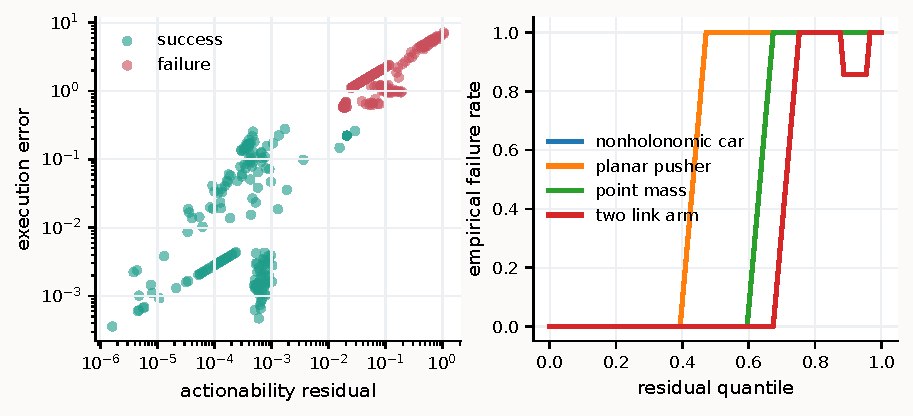
\includegraphics[width=0.9\linewidth]{figures/fig4_failure_prediction.pdf}
\caption{Actionability residuals correlate with rollout error and produce monotone failure-rate curves across embodiments.}
\label{fig:failure}
\end{figure}

\paragraph{Experiment 3: repair.}
We compare the original candidate, goal-only, world+goal, world+goal+smoothness, world+goal+actionability, and full energy variants. Adding actionability changes the trajectory rather than only rescoring it; it encourages futures whose local increments can be produced by bounded actions.

\begin{table}[t]
\centering
\caption{Repair success on diagnostic non-executable futures. The full energy includes world, goal, smoothness, and actionability terms.}
\label{tab:repair}
\begin{tabular}{lcc}\toprule
Environment & Candidate & Full energy\\\midrule
nonholonomic car & 0 & 1\\
planar pusher & 0 & 1\\
point mass & 0 & 1\\
two link arm & 0 & 1\\
\bottomrule\end{tabular}

\end{table}

\begin{figure}[t]
\centering
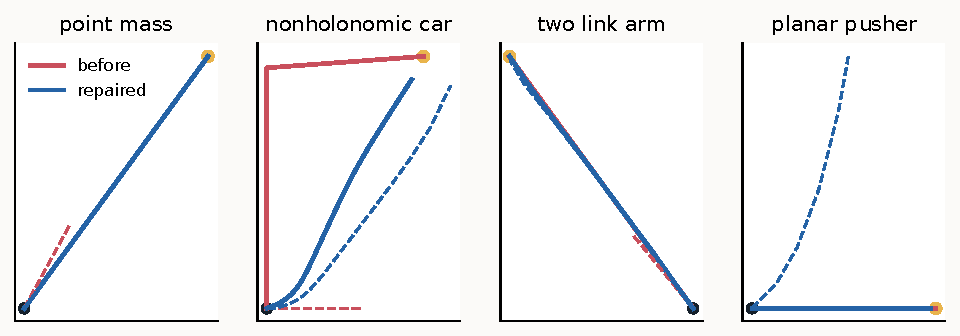
\includegraphics[width=0.95\linewidth]{figures/fig5_repair_before_after.pdf}
\caption{Before/after repair examples. Solid lines show imagined futures; dashed lines show rollouts from recovered controls.}
\label{fig:repair}
\end{figure}

\paragraph{Experiment 4: embodiment swap.}
We score the same local $(dx,dy)$ displacement under different action maps. The residual changes sharply across embodiments, showing that executability is body-conditioned.

\begin{figure}[t]
\centering
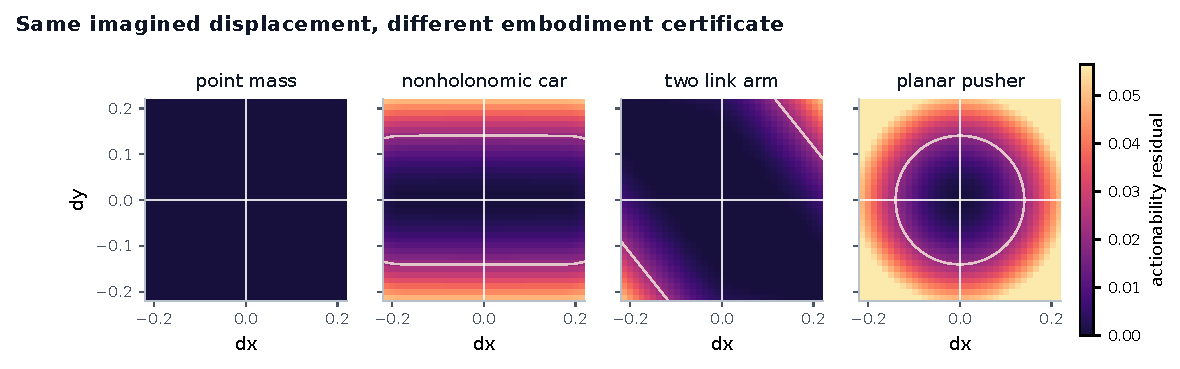
\includegraphics[width=0.95\linewidth]{figures/fig6_embodiment_swap.pdf}
\caption{Embodiment swap heatmaps. The same representation displacement can be actionable for one body and non-actionable for another.}
\label{fig:swap}
\end{figure}

\paragraph{Experiment 5: learned $J_\phi$.}
We fit small local linear action maps from random rollouts and compare them to analytic Jacobians. Error decreases with sample count, but the pusher remains harder because contact discontinuities violate a single smooth local model.

\begin{figure}[t]
\centering
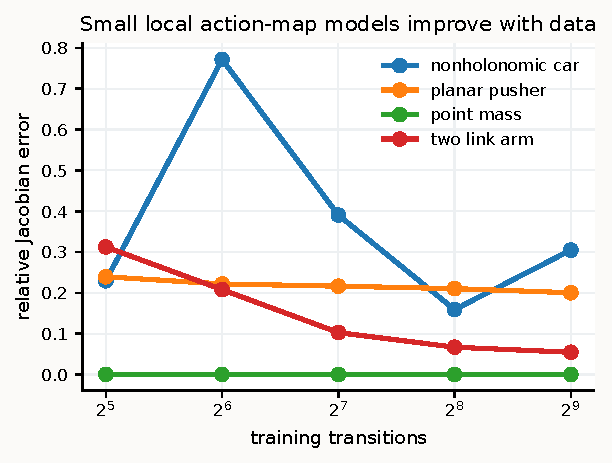
\includegraphics[width=0.52\linewidth]{figures/fig7_learned_jacobian.pdf}
\caption{Sample efficiency of small local action-map models.}
\label{fig:learnedj}
\end{figure}
